\subsubsection{Sensorem}

% \begin{wrapfigure}{r}{0.5\textwidth}
%     \centering
%     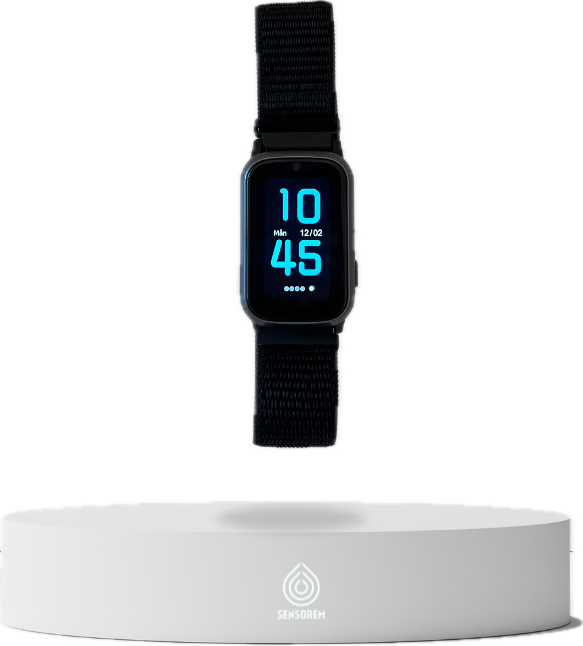
\includegraphics[width=0.5\linewidth]{report//images/sensorem.png}
%     \caption{Sensorem tryghedsalarm ("security alarm")}
%     \label{fig:sensorem_tryghedsalarm}
% \end{wrapfigure}



Sensorem (as seen in \autoref{fig:sensorem_tryghedsalarm}) is a Swedish company specializing in safety alarms for the elderly. The background of the company is the challenge faced by both Sweden and Denmark: a growing elderly population. Sensorem’s mission is to create solutions that provide seniors with greater safety in their daily lives, allowing them to stay in their own homes for as long as possible and, in many cases, completely avoid the need for a nursing home.

\wrapimage{r}
    {report//images/sensorem.png}
    {Sensorem tryghedsalarm ("security alarm")}
    {sensorem_tryghedsalarm}



The company has developed a discreet watch with an integrated alarm that is not visible. The watch has a button the user can press if they need help. In addition, it is equipped with an automatic fall detection system that registers if the user falls and immediately activates the alarm. In such cases, relatives are called through the watch’s built-in speakerphone.

The speakerphone makes it possible for relatives to communicate directly with the user via an app. If none of the relatives respond, Sensorem’s alarm center takes over and handles the situation.

The watch is connected to the mobile network, which means it works everywhere, even outside the home. Should an incident occur away from the user’s residence, the signal is still sent to the relatives. The watch is also equipped with \gls{gps}, so relatives can always see the user’s position in real time.

An important advantage is that the safety alarm does not require any connection to home care services. The alarm goes directly to the relatives. If the relatives do not respond, it is automatically forwarded to Sensorem’s alarm center, which can call an ambulance.

In addition to fall detection, the watch also features an inactivity alarm that notifies relatives if the watch has been inactive during selected time periods. This allows relatives to know if something has happened in situations where the user may not have been able to press the alarm button.

At the same time, the watch can also be used for medication reminders. These reminders are set up in the app, and the user receives notifications on the watch, both via text and voice.
